%%% Template originaly created by Karol Kozioł (mail@karol-koziol.net) and modified for ShareLaTeX use

\documentclass[a4paper,11pt]{article}
\usepackage{comment}
\usepackage[T1]{fontenc}
\usepackage[utf8]{inputenc}
\usepackage{graphicx}
\usepackage{xcolor}
\usepackage{hyperref}
\hypersetup{
    colorlinks=true,
    linkcolor=blue,
    filecolor=magenta,      
    urlcolor=cyan,
    citecolor=blue,
}


\renewcommand\familydefault{\sfdefault}
\usepackage{tgheros}
\usepackage[defaultmono]{droidmono}

\usepackage{amsmath,amssymb,amsthm,textcomp}
\usepackage{enumerate}
\usepackage{multicol}
\usepackage{tikz}

\usepackage{geometry}
\geometry{left=25mm,right=25mm,%
bindingoffset=0mm, top=20mm,bottom=20mm}


\linespread{1.3}

\newcommand{\linia}{\rule{\linewidth}{0.5pt}}

% custom theorems if needed
\newtheoremstyle{mytheor}
    {1ex}{1ex}{\normalfont}{0pt}{\scshape}{.}{1ex}
    {{\thmname{#1 }}{\thmnumber{#2}}{\thmnote{ (#3)}}}

\theoremstyle{mytheor}
\newtheorem{defi}{Definition}

% my own titles
\makeatletter
\renewcommand{\maketitle}{
\begin{center}
\vspace{2ex}
{\huge \textsc{\@title}}
\vspace{1ex}
\\
\linia\\
\@author \hfill \@date
\vspace{4ex}
\end{center}
}
\makeatother
%%%

% custom footers and headers
\usepackage{fancyhdr}
\pagestyle{fancy}
\lhead{}
\chead{}
\rhead{}
\lfoot{Integer Computation}
\cfoot{}
\rfoot{\thepage}
\renewcommand{\headrulewidth}{0pt}
\renewcommand{\footrulewidth}{0pt}
%

% code listing settings
\usepackage{listings}
\lstset{
    language=Python,
    basicstyle=\ttfamily\small,
    aboveskip={1.0\baselineskip},
    belowskip={1.0\baselineskip},
    columns=fixed,
    extendedchars=true,
    breaklines=true,
    tabsize=4,
    prebreak=\raisebox{0ex}[0ex][0ex]{\ensuremath{\hookleftarrow}},
    frame=lines,
    showtabs=false,
    showspaces=false,
    showstringspaces=false,
    keywordstyle=\color[rgb]{0.627,0.126,0.941},
    commentstyle=\color[rgb]{0.133,0.545,0.133},
    stringstyle=\color[rgb]{01,0,0},
    numbers=left,
    numberstyle=\small,
    stepnumber=1,
    numbersep=10pt,
    captionpos=t,
    escapeinside={\%*}{*)}
}

%%%----------%%%----------%%%----------%%%----------%%%

\begin{document}

\title{QI: Integer Computation: Factoring, Multiplication}

\author{Gregory Croisdale, Cade Brown, and Rebecca Ryan}

\date{\today}

\maketitle

\begin{center}
    This paper was written for PHYS494 at the University of Tennessee, Knoxville taught by George Siopsis in Spring, 2020.
\end{center}

\tableofcontents

\section{Abstract}
In this paper, we discuss some of the historically important quantum algorithms involving integers and their factors. We compare the feasibility and speed of some of the most impressive classical algorithms with our own implementation of the well-discussed "breaker of RSA": Shor's Algorithm\textsuperscript{\ref{sec:shor},\ref{sec:rsa}}. We describe attempts and problems with implementing the Lucas-Lehmer Primality Test\textsuperscript{\ref{sec:lehmer}} and the Fourier Transform for Multiplication\textsuperscript{\ref{sec:mult}}.


\section{Accompanying Materials}
The source code of all the algorithms we refer to in this paper can be found and ran from this GitHub Project:
\begin{center}
\url{https://github.com/gcrois/QFastInteger}.
\end{center}

A static version of the demo page is available for viewing at the following address:
\begin{center}
    \url{https://gcrois.github.io/QFastInteger/demo.html}.
\end{center}

\section{Introduction}\label{sec:intro}


\subsection{The Importance of Primes}
\cite{C5}\cite{Prime}\cite{QLect}
The current computer systems we have are due to the prime numbers.  Because prime numbers only have themselves and one as their factors, they are unique in the way that they cannot be broken down further while remaining a stable integer.  Therefore, prime numbers serve as the basis of encryption schemes, because they few and far between in comparison to composite numbers.  

\subsection{Encryption}
\cite{C5}\cite{QLect}\cite{Im}\cite{QCQI}
Encryption schemes are based heavily on prime numbers due to the fact that any two prime numbers multiplied together will ascertain a quick result, however, the reverse of this process is very labor intensive.  In order for the safest encryption, these primes must be truly random.  However, the prime numbers chosen must be somewhat related.  This relationship does decrease the security of the encryption, but is necessary when considering asymmetric cryptography.

\subsection{Error Correction}
\cite{C5}\cite{QLect}\cite{QCQI}\cite{Clone}
Error correction is required to ensure that the recipient receives uncorrupted data, that is, the original message has not been compromised.  In quantum error correction, the main culprits are decoherence and noise, which must be addressed in order for the system to be completely  fault-tolerant.  Classically, this is done by redundancy, however, due to the no-cloning theorem \cite{Clone} this is impossible because quantum computing processes are reversible. 


\subsection{The Importance of Factoring}
\cite{C5}\cite{QLect}
Factoring is important in order to determine the possible prime numbers p and q that were used in encrypting the original data, N.  In order to determine p and q, all of the prime factors of N must be found.  This is not a trivial process as p and q tend to be very large, in addition to showing an almost nonexistent correlation.  This could be done with more than two prime numbers, but for simplicity’s sake only two have been considered.  


\begin{comment}


\subsubsection{Greatest Common Denominator}

The greatest common denominator (gcd) of a set of integers is the largest number that divides evenly into all integers without a remainder.  For example, $gcd(35, 50) = 5$, where each factor can be broken down into smaller parts $(35 = 5^1 * 7; 50 = 5^2 * 2)$.  This is very important for decryption, as the gcd will help in breaking down the possible prime numbers that were used to encrypt data in the first place.  When prime numbers are raised to powers of prime numbers, that decreases the safety of the encryption which is why it is preferable to choose large prime numbers, without prime exponents, which are much harder to factor.  

\subsubsection{Least Common Multiple}
The least common multiple (lcm) is the smallest number that is divisible by two integers.  Specifically, it is the smallest number of prime factorizations of the gcd.  Taking the lcm and expressing it as prime powers is a way to calculate prime factorizations that would otherwise be harder to decrypt.  This follows the same logic as for determining a gcd, where too many prime options are discouraged due to ease of factorizability.


\end{comment}



\subsection{Importance of Fourier Transform}
\cite{Heat}\cite{FFTA}\cite{Probab}\cite{Harm}
The Fourier Transform (FT) is a mathematical relationship that allows for functions to be broken down into frequencies of sines and cosines, represented by a Fourier Series.  The combination of two functions f and g will produce two new functions (h and j), depending on whether f acts on g or g acts on f where f and g are sine or cosine functions.  The resultant is a transformation of the functions acting upon each other. 

\subsubsection{Convolution}
\cite{Asym}\cite{Qconvq}\cite{FFTA}
Convolution is where two functions acting upon each other produce a new function, based on a localized integral (or discrete summation in the case of discrete sequences). Essentially, you take two functions/sequences ($f$ and $g$), and their convolution (denoted $f * g$) is defined as the sum of values at different offsets, and the complete convolution is the set of all such points. So, for example, $f * g = [1, 0, 0, 2] * [4, 5] $, we can choose either $f$ or $g$ to make copies of, and then calculate the pointwise dotproduct of them shifted:

$[1, 0, 0, 2] * 4$

$[0, 1, 0, 0, 2] * 5$

Summing the entries (and filling in empty ones as $0$) yields:

$[4, 5, 0, 8, 10]$

This is an extremely important operation, in all sorts of fields from audio and video processing, to integer multiplication, and more.

As part of our research, we found that it is physically impossible to construct a quantum circuit to convolve 2 sequences \cite{qconv}, so we could obviously not implement such a functionality for our paper. The problem comes from the fact that multiplication of qubits (i.e. their spin) cannot be done with a unitary matrix, and therefore cannot be reversible.


\subsubsection{Trigonometric Parsing}
\cite{SF}
Trigonometric parsing is how the FT is able to break down a function into sines and cosines, which then require sound analysis of the Fourier Series.  This allows for each component to be broken down into fundamental harmonics, where each is a pythagorized set creating a new harmonic, known as the spectrum of the signal.  Each note is a combination of sines and cosines, of which vibrate at a specific frequency and allow the Fourier coefficients to be determined thus giving the amplitude of a longitudinal sound wave.  Each transformed peak corresponds to a specific amplitude on an FT graph, which gives a clear picture of the wave function required to create a specific sound.

\subsubsection{Image Processing}
\cite{Vision}\cite{PErr}\cite{Robo}\cite{Img}\cite{DIP}
The discrete fourier transform (DFT) takes a 2-Dimensional image, and calculates the product of the spatial domain and basis set.  The sum of all of these products will recreate the transformed image, which can be returned to the original image using the inverse fourier transform (IFT).  Increasing the dimensions of FT calculations will decrease the number of necessary computations.

\subsection{Shor's Algorithm}
\cite{C5}\cite{Prime}\cite{QCQI}\cite{DFa}
Shor’s Algorithm takes an input number N, and finds the prime factors (p, q) of N.  This implements polynomial time QFT to factor these integers.  Should a quantum computer be able to handle the stress, it would hypothetically be able to break RSA encryptions that are currently in place.  In general, N is odd, as N/2 should not be able to be broken down into powers of 2 or else there would be too many computational wrap-arounds without substantial remainders.  If N were to be even, the encryption would be much easier to break due to similarity in prime factors.  

\subsection{Lucas-Lehmer Prime Check}\label{sec:lehmer}
\cite{Prime}
The Lucas-Lehmer (LL) test is able to determine whether or not a Mersenne number $(2^n - 1)$ is a prime number where n must also be prime.  Because prime factoring is a very slow process, the guess and check method for determining a Mersenne prime is much faster, and thus saves time in prime finding.  This generation of prime numbers increases the speed in which prime numbers are determined, albeit not necessarily the prime factors of N specifically.  However, the LL test will bring us that much closer to determining possible prime factors.  


\section{RSA Encryption}\label{sec:rsa}

\cite{PCS} First, we define RSA as a secure algorithm for transmitting secret messages on unsecured channels by use of public and private keys. Every RSA keypair is generated from prime integers $p$ and $q$, some numbers are generated thusly:

$N=pq$ (the modulus)

$\phi(N) = \lambda = \mathrm{lcm}(p-1, q-1)$

$e = ($ a random number that is coprime to $\lambda)$

$d = e^{-1} (\mod \lambda)$ (i.e. $de = 1 (\mod \lambda)$)


Now, we can define key sets as:

public: $(N, e)$

private: $(N, d)$

The public key can be freely distributed harmlessly to anyone on the planet. They can use it to encrypt messages and then send that encrypted data across the internet.

However, the only person which can decrypt and read the message is the one in possession of the private key. They can receive the encrypted data and then decrypt it using their privately held key.

\subsection{Sending And Receiving Messages}

The process for sending encrypted data begins with generating it:

Say we want to send a message (called $m$):

We generate the encrypted data:

$m_{enc} = m ^ e (\mod N)$

Then, the receiver with the private key calculates:

$m_{dec} = m_{enc} ^ d (\mod N) = (m ^ e) ^ d (\mod N) = m ^ {e * d} (\mod N)$

And, it can be shown that for any number, $a^i = a^{i \mod \phi(N)} (\mod N)$ for any $a, i, N$.

And, since we know that $e * d = 1 (\mod \phi(N))$, the above can be simplified to:

$m_{dec} = m ^ {e * d \mod \phi(N)} (\mod N) = m ^ {1} (\mod N) = m$

And, thus, the decrypted message is equal to the original message $m$

\subsection{Breaking RSA}

To break RSA, we would like to factor the number $N$ (which is included with both the public and private keypairs). Obviously, factoring integers is hard. A brute force method for finding a factor of $n$ is located below:

\begin{lstlisting}
def factor(n):
    # small cases outside the (2#) wheel
    if n % 2 == 0: return 2
    if n % 3 == 0: return 3
    
    # upper bound on unique factors
    r = int(n ** 0.5)
    
    # check divisibility by (6k-1) and (6k+1) residues
    i = 5
    while i <= r:
        if n % i == 0: return i
        if n % (i + 2) == 0: return i + 2
        
        i += 6
    # no factors; n is prime
    return None
\end{lstlisting}


The code uses wheel factorization (i.e. only checking residue classes modulo $2\#=2*3=6$, which are $\{1, -1\}$) and a few special cases to isolate factors which occur in the first wheel.

This is not the best that can be done classically, but algorithms such as the GNFS are out of reach for this paper. Instead, we will focus on Quantum algorithms for breaking encryption (specifically, Shor's)

\subsection{Shor's Algorithm}\label{sec:shor}

Shor's algorithm is perhaps one of the most anticipated quantum algorithms, for the risk it poses to encryption (see above in the document), as well as the interesting result that drastically improves the computational complexity of integer factorization, a very interesting problem.

This algorithm will be interesting to implement, because it uses elements such as QFT, as well as partial computation on classical and quantum systems, which combine to solve the problem in polynomial time: $O(N^2 \log N \log \log N)$ (where $N$ is the size of the input).

An overview of Shor's algorithm is (to factor an integer $N$):

1. Pick a random number $1 < a < N$

2. If $\gcd(a, N) \neq 1$, then we have found a factor of $N$, so return that as a factor

3. Now, load a program on a quantum computer to 


While probabilistic algorithms already exist for primality testing on classical computers, finding out which numbers divide another number is still a very hard to solve problem using solely classical computers.

Shor's algorithm: \href{https://qudev.phys.ethz.ch/static/content/QSIT15/Shors\%20Algorithm.pdf}{https://qudev.phys.ethz.ch/static/content/QSIT15/Shors\%20Algorithm.pdf}

Our implementation, while working, has a few evident flaws. Firstly, our implementation does not use an efficient GCD or Inverse Modulo algorithm. This significantly hurts the runtime of the implementation. Additionally, as the quantum circuit is only being simulated, we do not see runtimes consistent with the proposed Big-O. When using the numpy version of fft, we see better times for this reason.

Shor's algorithm relies on a version of the FFT that works well on quantum circuits, as opposed to the problem of general convolution. Other algorithms that are able to utilize this less-than-ideal fact see theoretically tremendous speed-ups when viewed from a quantum standpoint.

It is also important to note that Shor's is not even the fastest quantum factoring algorithm, it was just the first substantial speed up. The \href{https://eprint.iacr.org/2017/351.pdf}{GEECM algorithm} allegedly is "much faster than Shor's". Regardless, this algorithm will always be historically significant as it captured the attention of all who were cryptographically aware - if RSA could be broken in polynomial time, could classical computers even safely send private information? For the time being, it seems that RSA keys greater than 10 bits are safe from our implementation.



\section{Fast Fourier Transform (FFT) Based Integer Multiplication}\label{sec:mult}

Integers can be multiplied quickly using FFT (Fast Fourier Transform) and convolution along their digits. This provides a monumental speedup as opposed to the naive complexity of $O(N^2)$ and some other algorithms (Katatsuba: $O(N^{1.58})$). Specifically, the FFT can yield theoretical algorithms of complexity $O(N \log N)$, a monumental speedup at larger values.

Integer multiplication of 2 integers ($A$ and $B$), which have base-$d$ 'digits' (not necessarily base 10) $a_0, ..., a_{N-1}$ such that $\sum_{i=0}^{N-1} a_i d^i = A$ and $b_0, ..., b_{N-1}$ such that $\sum_{i=0}^{N-1} b_i d^i = B$ have the result (we'll call it $C$) with $2*N$ 'digits'.

The formula for any given digit of 'C' (not accounting for overflow) is: $C_i=\sum_{j=0}^{i} a_{j}c_{i-j}d^{i}$

Thus, in the following vector-vector product: $ab^T$:
\newcommand\GREEN{\color{violet}}
\newcommand\BLUE{\color{blue}}

$$ \begin{bmatrix}
\BLUE a_0 b_0 & \GREEN a_0 b_1 & ... & a_0 b_{N-1} \\
\GREEN a_1 b_0 & a_1 b_1 & ... & a_1 b_{N-1} \\
... & ... & ... & ... \\
a_{N-1} b_0 & a_{N-1} b_1 & ... & a_{N-1} b_{N-1} \\
\end{bmatrix} $$


Each cross-diagonal sum will give the corresponding entry of $c$

Thus, $\BLUE c_0 = a_0 b_0$ and $\GREEN c_1 = a_0 b_1 + a_1 b_0$, and so on

Obviously, directly summing these entries yields a complexity of $O(N^2)$. However, there is a quicker way to do convolution for two 1-dimensional sequences, using the Fast Fourier Transform (FFT).

The formula is: $A*B=\textrm{IFFT}(\textrm{FFT}(a) \odot \textrm{FFT}(b))$

Where IFFT is the Inverse Fast Fourier Transform, and $\odot$ means pointwise multiplication. Using the Cooley-Tukey FFT algorithm (standard, and plenty of packages already implement this), the complexity is reduced to $O(3N \log N + N) = O(N \log N)$ (since point-wise multiplication of small elements is $O(N)$). This is the drastic speedup that allows faster integer multiplication.

We implemented this in Python (so, there were inefficiencies), but we did get an approximately correct complexity of runtime (albeit much slower than would be possible in C or some lower language). We show the time (in seconds) required for an $NxN$ bit multiplication (N=0 through 160000)

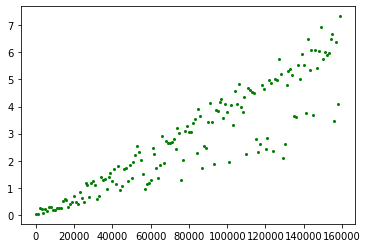
\includegraphics{intMM_time}

We also tried to implement it as a Quantum circuit. However, we soon researched and found out that this is impossible for the general case \cite{qconv} because of the pointwise multiplication of the FFT results. The reason for this is that a quantum gate that could perform multiplication of the state of 2 qubits would be non-unitary and thus irreversible, and therefore would not work. So, this method of integer multiplication is impossible to implement on a quantum computer.



\section{Conclusion}
When we first set out on this project, we intended to implement all of the aforementioned algorithms with quantum circuits. The lack of general convolution, however, made this prove to be impossible. Regardless, a lot of insight was gained. For the time being, it seems that the centuries of classical thinking have overwhelmed the few novel quantum circuits. With algorithms such as GEECM beginning to pop up and physical breakthroughs leading to greater feasibility of quantum computing, we think that quantum supremacy will soon, less controversially, be found.

The vast classical toolkit will soon have to compete with real implementations of algorithms which are orders of magnitude faster. One of the greatest advantages that classical computing has is the presence of average-case speedups and case switching - i.e., conditional shortcuts. These are easy to find and understand - for example, ignoring precision not required for the final answer in intermediate steps. These speedups may be possible in the realm of quantum computing, but they are much more difficult to find with our current understanding. Additionally, classical computing has a vast array of literature regarding computability. If you are approached with a problem, you can relatively easily determine if it is possible to find an answer and even how long it will take. This is not so easy with quantum - some operations which we take for granted are covertly difficult or even impossible with a quantum circuit (for example in our case, general convolution using a FT).

\begin{thebibliography}{9}
\bibitem{qconv} 
Lomont, C.
\textit{Quantum convolution and quantum correlation algorithms are physically impossible}.
\begin{verbatim}
https://www.researchgate.net/publication/2191142_Quantum_convolution_
and_quantum_correlation_algorithms_are_physically_impossible.
2003.
\end{verbatim}

\bibitem{Parity} 
Afflick, D.
\textit{“Parity Error Checking”}.
2020.

\bibitem{Vision} 
Ballard, D, Brown, C.
\textit{\emph{Computer Vision}, Prentice-Hall, 1982, pp 24-30.}

\bibitem{C5} 
BerkeleyX.
\textit{“Chapter 5: QFT, Period Finding, Shor’s Algorithm”, pp 49-68.}.

\bibitem{Prime} 
Crandall, R, Pomerance, C.
\textit{“Prime Numbers: A Computational Perspective” Springer 2001, pp 191-226.}.

\bibitem{QLect} 
de Wolf, R.
\textit{“Quantum Computing Lecture Notes”, 2012, pp 19-29}.

\bibitem{Primality} 
Donis-Vela, A, Garcia-Escartin, J.C.
\textit{“A quantum primality test with order finding” Quantum Information and Computation, 2018, Vol 18, 13-14}.

\bibitem{Heat} 
Fourier, JBJ.
\textit{“The Analytical Theory of Heat” University Press, 1878, pg. 166-209}.

\bibitem{Im} 
Goldreich, O.
\textit{Digital Image Processing, Addison-Wesley Publishing Company, 1992, pp 81-125.}

\bibitem{PErr} https://www.overleaf.com/project/5e63e283b86d04000152fd6c
Gonzales, R, Woods, R.
\textit{“Parity Error Checking”}.

\bibitem{MMult} 
Harnett, K.
\textit{“Mathematicians Discover the Perfect Way to Multiply” Quanta Magazine, 2019}.

\bibitem{Robo} 
Horn, B.
\textit{Robot Vision, MIT Press, 1986, Ch. 6-7}.

\bibitem{Img} 
Jain, A.
\textit{Fundamentals of Digital Image Processing, Prentice-Hall, 1989, pp 15-20.}

\bibitem{Harm} 
Katznelson, Y.
\textit{“An Introduction to Harmonic Analysis” 1976.}

\bibitem{Probab} 
Keller, W
\textit{An Introduction to Probability Theory and its Applications, 1971, Vol 2}.

\bibitem{SF} 
Kessler, B
\textit{"A "Sound" Approach to Fourier Transforms: Using Music to Teach Trigonometry" 2007 Bridges Donostia Conference Proceedings, 2007, 135-142}.

\bibitem{Asym} 
Li, B, Babu, GJ
\textit{“Convolution Theorem and Asymptotic Efficiency” A Graduate Course on Statistical Interference, Springer. 2019, pp. 259-327}.

\bibitem{Shora} 
Lin, FX
\textit{“Shor’s Algorithm and the Quantum Fourier Transform” Quantum Mechanics and Quantum Computation, 2016, pp 1-16}.

\bibitem{Qconvq} 
Lomont, C.
\textit{“Quantum convolution and quantum correlation algorithms are physically impossible”  Quantum Physics, 2003, pp 1-10}.

\bibitem{DIP} 
Marion, A.
\textit{An Introduction to Digital Image Processing, Chapman and Hall, 1991, Ch. 9.}

\bibitem{QCQI} 
Nielsen, MA, Chuang, IL.
\textit{“Quantum Computation and Quantum Information”, Cambridge University Press, 2000}.

\bibitem{FFTA} 
Osgood, B.
\textit{“The Fourier Transform and its Applications” Stanford Univ, 2007.}

\bibitem{PCS} 
Rivest, R, Shamir, A, Adleman, L.
\textit{“A Method for Obtaining Digital Signatures and Public-Key Cryptosystems” Communications of the ACM, 1978, pp 120-126}.

\bibitem{DFa} 
Shor, P.
\textit{“Algorithms for quantum computation: discrete logarithms and factoring”, 35th Annual Symposium on Foundations of Computer Science, 1994, 124-134}.

\bibitem{Clone} 
Wootters, W, Zurek, W.
\textit{“A Single Quantum Cannot be Cloned”, Nature 1982, pp 802-803}
2020.

\end{thebibliography}

\end{document}
